\documentclass[a4paper, 11pt, oneside]{article}

\usepackage[utf8]{inputenc}
\usepackage[T1]{fontenc}
\usepackage[english]{babel}
\usepackage{array}
\usepackage{shortvrb}
\usepackage{listings}
\usepackage[fleqn]{amsmath}
\usepackage{amsfonts}
\usepackage{fullpage}
\usepackage{enumerate}
\usepackage{enumitem}
\usepackage{graphicx}
\usepackage{subfigure}
\usepackage{alltt}
\usepackage{indentfirst}
\usepackage{eurosym}
\usepackage{listings}
\usepackage{titlesec, blindtext, color}
\usepackage{float}
\usepackage[colorlinks, linkcolor=blue]{hyperref}
\usepackage[nameinlink,noabbrev]{cleveref}

\usepackage{titling}
\renewcommand\maketitlehooka{\null\mbox{}\vfill}
\renewcommand\maketitlehookd{\vfill\null}

\definecolor{mygray}{rgb}{0.5,0.5,0.5}
\definecolor{pink1}{rgb}{0.858, 0.188, 0.478}
\definecolor{sienna}{rgb}{0.53, 0.18, 0.09}
\definecolor{sepia}{rgb}{0.44, 0.26, 0.08}
\definecolor{midnightblue}{rgb}{0.1, 0.1, 0.44}

\lstset{
    language=C, % Utilisation du langage C
    commentstyle={\color{midnightblue}}, % Couleur des commentaires
    frame=single, % Entoure le code d'un joli cadre
    rulecolor=\color{black}, % Couleur de la ligne qui forme le cadre
    stringstyle=\color{sienna}, % Couleur des chaines de caractères
    % numbers=left, % Ajoute une numérotation des lignes à gauche
    numbersep=5pt, % Distance entre les numérots de lignes et le code
    numberstyle=\tiny\color{mygray}, % Couleur des numéros de lignes
    basicstyle=\tt\footnotesize, 
    tabsize=3, % Largeur des tabulations par défaut
    keywordstyle=\tt\bf\footnotesize\color{sepia}, % Style des mots-clés
    extendedchars=true, 
    captionpos=b, % sets the caption-position to bottom
    texcl=true, % Commentaires sur une ligne interprétés en Latex
    showstringspaces=false, % Ne montre pas les espace dans les chaines de caractères
    escapeinside={(>}{<)}, % Permet de mettre du latex entre des <( et )>.
    inputencoding=utf8,
    literate=
  {á}{{\'a}}1 {é}{{\'e}}1 {í}{{\'i}}1 {ó}{{\'o}}1 {ú}{{\'u}}1
  {Á}{{\'A}}1 {É}{{\'E}}1 {Í}{{\'I}}1 {Ó}{{\'O}}1 {Ú}{{\'U}}1
  {à}{{\`a}}1 {è}{{\`e}}1 {ì}{{\`i}}1 {ò}{{\`o}}1 {ù}{{\`u}}1
  {À}{{\`A}}1 {È}{{\`E}}1 {Ì}{{\`I}}1 {Ò}{{\`O}}1 {Ù}{{\`U}}1
  {ä}{{\"a}}1 {ë}{{\"e}}1 {ï}{{\"i}}1 {ö}{{\"o}}1 {ü}{{\"u}}1
  {Ä}{{\"A}}1 {Ë}{{\"E}}1 {Ï}{{\"I}}1 {Ö}{{\"O}}1 {Ü}{{\"U}}1
  {â}{{\^a}}1 {ê}{{\^e}}1 {î}{{\^i}}1 {ô}{{\^o}}1 {û}{{\^u}}1
  {Â}{{\^A}}1 {Ê}{{\^E}}1 {Î}{{\^I}}1 {Ô}{{\^O}}1 {Û}{{\^U}}1
  {œ}{{\oe}}1 {Œ}{{\OE}}1 {æ}{{\ae}}1 {Æ}{{\AE}}1 {ß}{{\ss}}1
  {ű}{{\H{u}}}1 {Ű}{{\H{U}}}1 {ő}{{\H{o}}}1 {Ő}{{\H{O}}}1
  {ç}{{\c c}}1 {Ç}{{\c C}}1 {ø}{{\o}}1 {å}{{\r a}}1 {Å}{{\r A}}1
  {€}{{\euro}}1 {£}{{\pounds}}1 {«}{{\guillemotleft}}1
  {»}{{\guillemotright}}1 {ñ}{{\~n}}1 {Ñ}{{\~N}}1 {¿}{{?`}}1
}


\newcommand{\ClassName}{INFO-2055: Embedded systems project}
\newcommand{\ProjectName}{Customer Counter\\Sensors and actuators validation}
\newcommand{\AcademicYear}{2020 - 2021}

%%%% Page de garde %%%%

\title{\ClassName\\\vspace*{0.8cm}\ProjectName\vspace{0.8cm}}
\author{Crucifix Arnaud \\170962 \and Goffart Maxime \\180521 \and Joris Olivier \\ 182113}
\date{\vspace{1cm}Academic year \AcademicYear}

\begin{document}

%%% Page de garde %%%
\begin{titlingpage}
{\let\newpage\relax\maketitle}
\end{titlingpage}

%%%%%%%%%%%%%%%%%%%%%%%%%%%%%%%%%%%%%%%%%%%%%%

\section{Project idea \small{(reminder)}}

We are going to use a microcontroller to manage the maximum number of customers allowed inside a shop in this period of health crisis. \par
Indeed, it will keep track of the number of persons allowed inside the shop. We will use an infrared sensor system to detect customers entering and leaving the shop. In order to limit the customers' flow, we will use 7 segments to display the number of customers that can still enter. When powering up the system or after a reset, we will also use these 7 segments displays to configure the maximum number of customers that can be in the shop at the same time using buttons.

%%%%%%%%%%%%%%%%%%%%%%%%%%%%%%%%%%%%%%%%%%%%%%

\section{Hardware \small{(updated)}}
We are using one infrared emitter for the entry and another one for the exit. Moreover, we are using a "central" circuit that will contain both receivers. Thus, we have 2 different kinds of circuits.\par
Thanks to this choice, we can choose how far we want each emitter to be from the receiving circuit as long as we stay in the limit of the emitters.

\subsection{Schematic}
The main modifications, compared to the previous circuit, are splitting the emitting and receiving parts and switching to 9V battery as a power source instead of 5V DC power supply using a jack connector.

\subsubsection{Receiver}
The receiving circuit contains both infrared receivers, both 7 segments, and buttons to set the limit of customers. Moreover, the LED D1 will be blinking while the manager chooses the maximum number of customers and staying switched on when the system is operational. See \autoref{fig:receiver} for the schematic.
\begin{figure}[p]
    \centering
    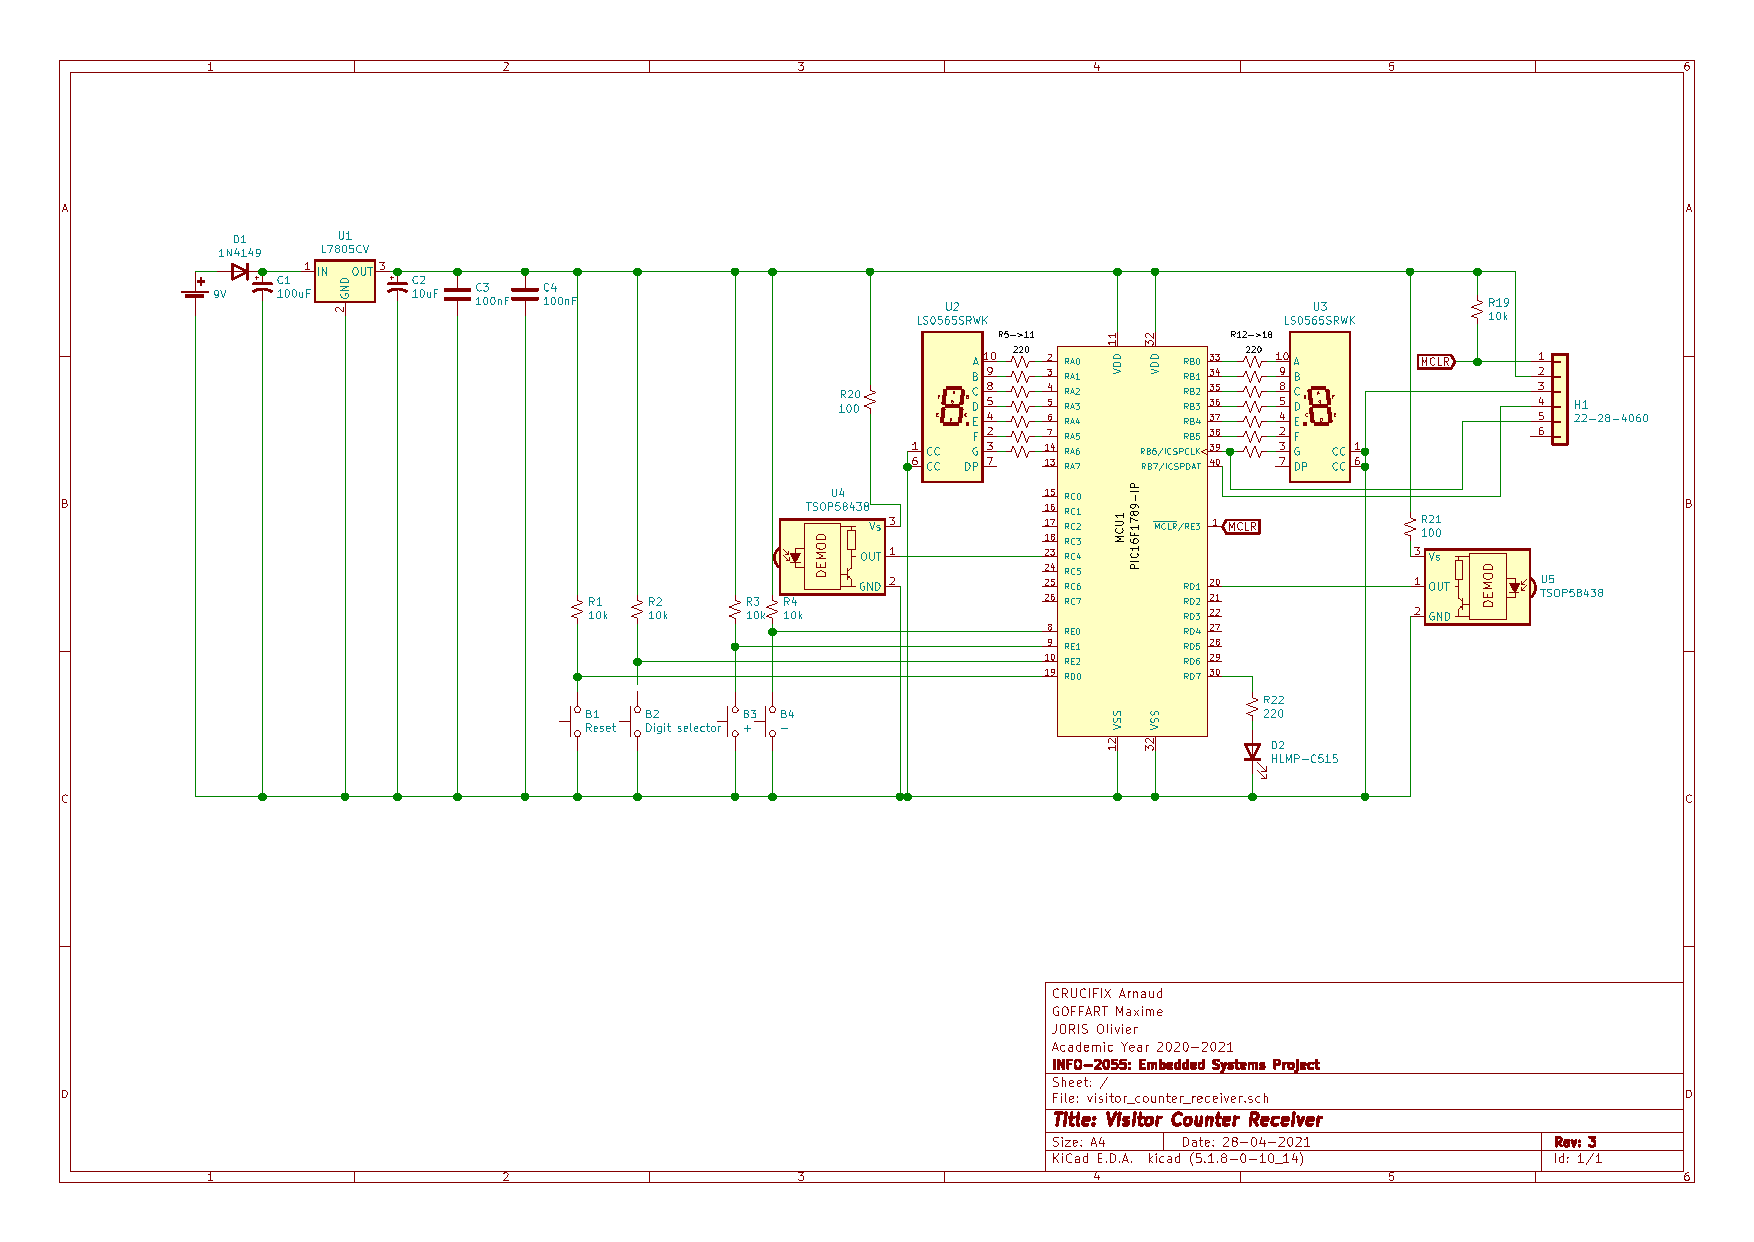
\includegraphics[angle=90, scale=0.75]{visitor_counter_receiver.pdf}
    \caption{Schematic of the receiving circuit}\label{fig:receiver}
\end{figure}

\subsubsection{Emitter}
Each emitting circuit contains an infrared emitter with secondary components in order to regulate the voltage. See \autoref{fig:emitter} for the schematic.
\begin{figure}[p]
    \centering
    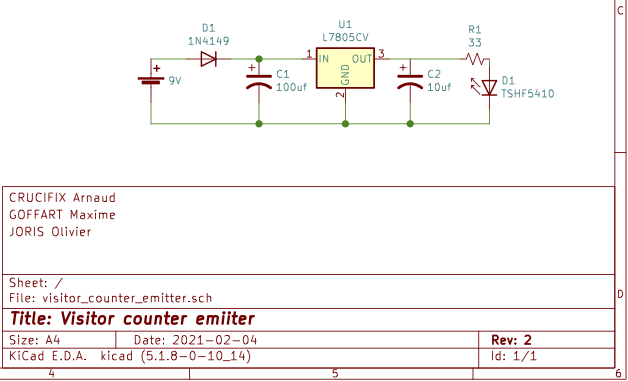
\includegraphics[angle=90, scale=0.75]{visitor_counter_emitter.png}
    \caption{Schematic of the emitting circuit}\label{fig:emitter}
\end{figure}

\subsection{Physical circuit}
We will setup the system in the following way:
\begin{figure}[H]
    \centering
    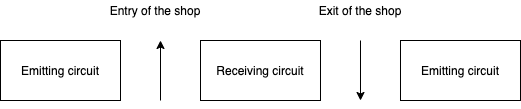
\includegraphics[scale=0.75]{diagram.png}
    \caption{Abstract representation of the setup of the 3 circuits}
\end{figure}
The 3 circuits will have to be at a certain height in order to improve the detection. A trial-and-error method must be used in order to determine the optimal height.


%%%%%%%%%%%%%%%%%%%%%%%%%%%%%%%%%%%%%%%%%%%%%%

%%%%%%%%%%%%%%%%%%%%%%%%%%%% STATES FOR TESTING %%%%%%%%%%%%%%%%%%%%%%%%%%%%
% First, test the IR receivers
% Then , test the 2x 7 segments
% Buttons can be pushed at any time EXCEPT when testing the IR receivers
%   (do not react to change of voltages on the input
%    of the buttons during the first phase)
%
% The LED D1 should be turned off by default
%
% Consider the current schematic for the ports
% If needed, I will modify the code (if I change the ports)
%%%%%%%%%%%%%%%%%%%%%%%%%%%%%%%%%%%%%%%%%%%%%%%%%%%%%%%%%%%%%%%%%%%%%%%%%%%%%

\section{Sensors}
\textbf{TO BE FILLED}

\subsection{Infra-red receivers}
\textbf{TO BE FILLED} \par
Idea of test: if someone (or just an object) is detected by the sensor, light up the green LED of the receiver (D1 on the schematic).

\subsection{Buttons}
\textbf{TO BE FILLED} \par
Idea of test: if someone press one of the button, light up the green LED of the receiver (D1 on the schematic).

%%%%%%%%%%%%%%%%%%%%%%%%%%%%%%%%%%%%%%%%%%%%%%

\section{Actuators}
\paragraph{}\textbf{TO BE FILLED}

\subsection{7 segments}
\textbf{TO BE FILLED} \par
Idea of test: display 11, 22, 33, 44, 55, 66, ..., up to 99. With a 2 seconds delay between switching between 2 numbers (with interrupts).

\subsection{LEDs}
\textbf{TO BE FILLED} \par
Already tested before.

%%%%%%%%%%%%%%%%%%%%%%%%%%%%%%%%%%%%%%%%%%%%%%

\section{Software}
\textbf{TO BE FILLED} \par
\textit{Add code being used for the tests}.

\end{document}
